\documentclass[UTF8]{ctexart}
\ctexset { section = { format={\Large \bfseries } } }
\pagestyle{plain}
\usepackage{float}
\usepackage{amsmath}
\usepackage{amssymb}
\usepackage{listings}
\usepackage{subfigure}%1并排图片宏包
\usepackage{graphicx}%插入图片宏包
\usepackage{xcolor}
\usepackage{geometry}
\geometry{a4paper,scale=0.8}
\usepackage{caption}
\captionsetup[figure]{name={Figure}}
\captionsetup[table]{name={Table}}


\lstset{
language=Python, % 设置语言
basicstyle=\ttfamily, % 设置字体族
breaklines=true, % 自动换行
keywordstyle=\bfseries\color{blue}, % 设置关键字为粗体,
morekeywords={}, % 设置更多的关键字,用逗号分隔
emph={self}, % 指定强调词,如果有多个,用逗号隔开
emphstyle=\bfseries\color{Rhodamine}, % 强调词样式设置
commentstyle=\color{black!50!white}, % 设置注释样式,斜体,浅灰色
stringstyle=\bfseries\color{red!90!black}, % 设置字符串样式
columns=flexible,
numbers=left, % 显示行号在左边
numbersep=2em, % 设置行号的具体位置
numberstyle=\footnotesize, % 缩小行号
frame=single, % 边框
framesep=1em % 设置代码与边框的距离
}

\title{\textbf{Image Processing Homework 1}}
\author{吴嘉骜 21307130203}
\date{\today}

\begin{document}

\maketitle

\noindent
\section{}
\setlength{\parindent}{0pt}
Implement a piecewise linear transformation function for image contrast stretching. The code should read in an image; 
for intensity of all pixels, use the function to compute new intensity values; and finally output / save the image with new intensity values.\\
\textbf{Solution}: See piecewiselinear\_img.py
\begin{lstlisting}
from PIL import Image

def piecewise_linear_transformation(img_path, r1, s1, r2, s2, L=256):
    
    '''
    Apply piecewise linear transformation for contrast stretching.
    
    Parameters:
        - img_path: path to input image.
        - r: input intensities.
        - s: output intensities.
        - r1, s1: First location point.
        - r2, s2: Second location point.
            Generally, r1<=r2 and s1<=s2.
        - L: Number of intensity levels, default is 256.
    Returns:
        - None. Saves the image and prints the path.
    '''

    # open image
    img = Image.open(img_path)
    
    # convert to grayscale if not already
    if img.mode != 'L':
        img = img.convert('L')

    # define piecewise linear function
    def transform_function(r,r1,r2,L):
        if r1 == 0:
            r1 = 1
        if r2 == L-1:
            r2 = L-2 # to avoid division by zero
        if r1 == r2:
            if 0 <= r < r1:
                s = round((s1 / r1) * r)
            else:
                s = round(((L-1 - s2) / (L-1 - r2)) * (r - r2) + s2)
        else:
            if 0 <= r < r1:
                s = round((s1 / r1) * r)
            elif r1 <= r <= r2:
                s = round(((s2 - s1) / (r2 - r1)) * (r - r1) + s1)
            else:
                s = round(((L-1 - s2) / (L-1 - r2)) * (r - r2) + s2)
        
        if s > L-1: # clamp to L-1
            return L-1
        else:
            return s
    
    # apply the function to every pixel value
    pixels = img.load()
    for i in range(img.width):
        for j in range(img.height):
            intensity = pixels[i, j]
            pixels[i, j] = transform_function(intensity,r1,r2,L)

    # save the modified image
    img_out_path = "piecewise_image.jpg"
    img.save(img_out_path)

    print(f"Image saved at {img_out_path}")
    
# Test the function
input_image_path = '.\HW1\pollen.tif'
img1 = Image.open(input_image_path)
pixels = img1.load()
maxr = -99
minr = 100
for i in range(img1.width):
    for j in range(img1.height):
        intensity = pixels[i, j]
        if intensity > maxr:
            maxr = intensity
        if intensity < minr:
            minr = intensity
print(minr,maxr)

piecewise_linear_transformation(input_image_path, minr, 0, maxr, 255)
\end{lstlisting}
\textbf{Code interpretation}:\\
The code above defines a piecewise linear transformation function for image contrast stretching. The function takes in an image path, together with location points $r_1, s_1, r_2, s_2$ and the number of intensity levels $L$.
The function first opens the image, then defines the piecewise linear function and applies it to every pixel value. To avoid division by zero, the function checks if $r_1$ or $r_2$ is equal to 0 or $L-1$. If so, it changes the value to 1 or $L-2$ respectively.
Then it checks if $r_1$ is equal to $r_2$. If not, it applies the function according to the formula in the question.
Finally, it saves the modified image and prints the path.\\
\textbf{Result}:\\
The input original image and the output image after piecewise linear transformation are shown below. The enhanced figure is obtained by setting $(r_1,s_1)=(r_{min},0),\, (r_2,s_2)=(r_{max},L-1)$
where $r_{min}$ and $r_{max}$ denote the minimum and maximum intensity levels in the input image.
We can see that the contrast of the image is enhanced after piecewise linear transformation. Object contours and surface details become clearer.
\begin{figure}[htbp]	
	\subfigure[Input original image] %第一张子图
	{
		\begin{minipage}{8cm}
			\centering          %子图居中
			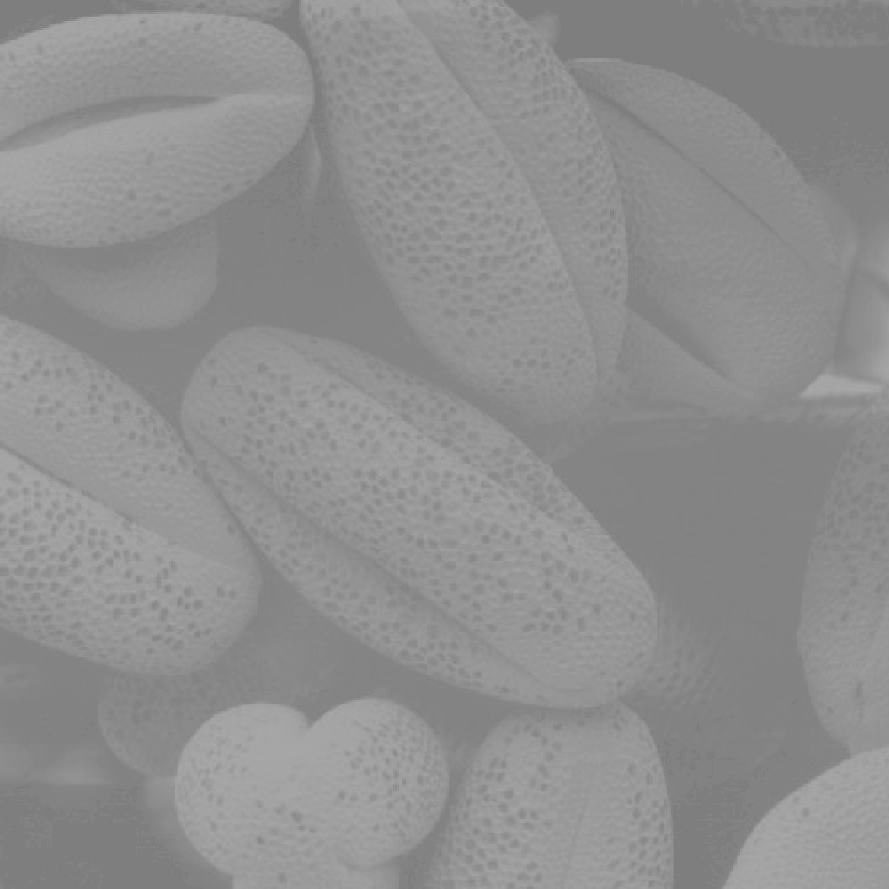
\includegraphics[scale=0.15]{pollen.jpg} 
		\end{minipage}
	}
	\subfigure[Output image after transformation] %第二张子图
	{
		\begin{minipage}{8cm}
			\centering      %子图居中
			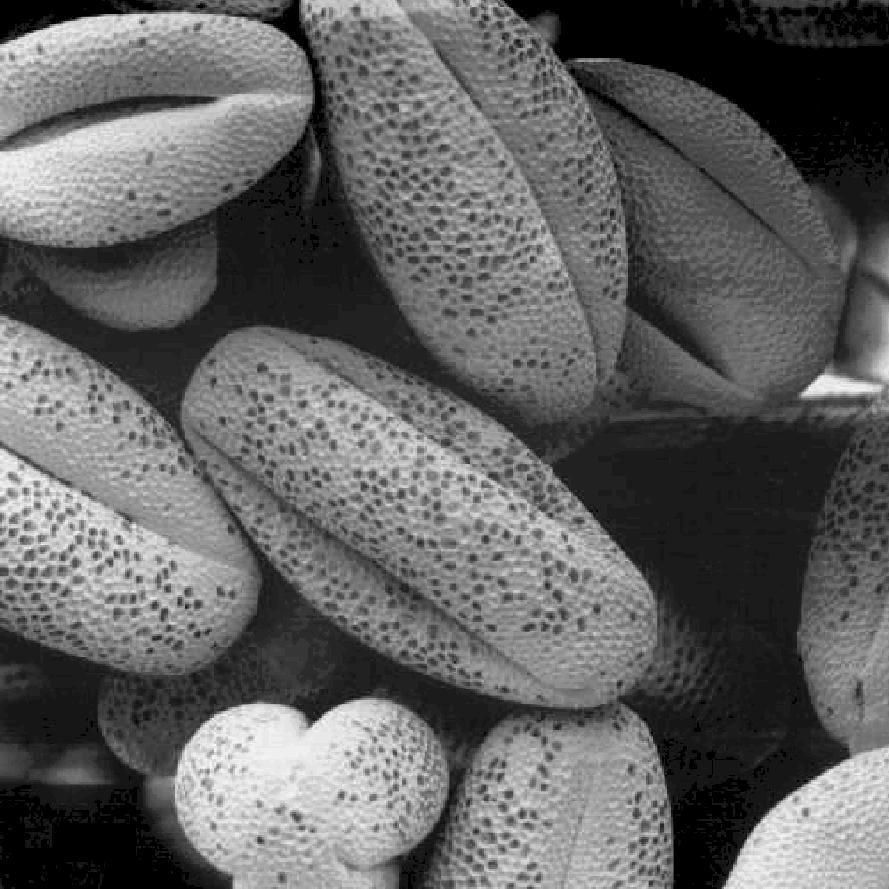
\includegraphics[scale=0.15]{piecewise_transed.jpg}
		\end{minipage}
	}
	\caption{Image after piecewise linear transformation} %  %大图名称
\end{figure}


\section{}
(1) Implement $n$-dimensional joint histogram and test the code on two-dimensional data; plot the results.\\
(2) Implement computation of local histograms of an image using the efficient update of local histogram method introduced in local histogram processing.\\
Note that because only one row or column of the neighborhood changes in a one-pixel translation of the neighborhood, updating the histogram obtained in the previous location with the new data introduced at each motion step is possible and efficient in computation.\\
\textbf{Solution}:\\
(1) See joint\_histogram.py
\begin{lstlisting}
import numpy as np

def evaluate_histogram(data_np, no_bins, data_min, data_max):
    """
    Evaluate an n-dimensional histogram.
    
    Parameters:
        - data_np: np.ndarray of shape (dimension, data)
        - no_bins: list of bins count for each dimension
        - data_min: list of minimum for each dimension
        - data_max: list of maximum for each dimension

    Returns:
        - histogram: np.ndarray of shape specified by no_bins
    """

    dimension = data_np.shape[0]
    numdata = data_np.shape[1] # Number of data points
    
    # Initialize histogram, an all-zero n-D array of size no_bins
    histogram = np.zeros(tuple(no_bins), dtype=int)
    
    # Compute bin spacings for each dimension
    bin_spacings = [(data_max[i] - data_min[i]) / no_bins[i] for i in range(dimension)]
    
    # Compute bin position for each point in data and increment histogram count
    for i_data in range(numdata):  # Loop over data points
        bin_pos = []  # Bin position for this data point
        for i_dim in range(dimension):  # Loop over dimensions
            value = data_np[i_dim][i_data]
            b = int((value - data_min[i_dim]) / bin_spacings[i_dim])  # Bin index
            # Prevent out-of-bound indices
            b = max(b, 0)
            b = min(b, no_bins[i_dim] - 1)
            bin_pos.append(b)
        
        # Increment histogram count at the computed position
        histogram[tuple(bin_pos)] += 1
    
    return histogram


def bins_power_of_two(n):
    
    """
    Determine number of bins as a power of 2.
    """
    k = np.log2(np.log2(n))
    
    return int(2**np.ceil(k))
\end{lstlisting}
\textbf{Code interpretation}:\\
The code above defines a function to evaluate an $n$-dimensional histogram. 
The function takes in an $n$-dimensional data array, a list of bins count for each dimension, a list of minimum for each dimension and a list of maximum for each dimension (could be a close guess). 
For the number of bins, we use an empirical result that it should be a power of 2, and closed to $logN$.\\
The function first initializes an all-zero $n$-dimensional array of size no\_bins, then computes bin spacings for each dimension. Finally, it computes bin position for each point in data and increments histogram count.
If the bin index is out of bound, it clamps the index to the leftmost or rightmost bin. We can use an $n$-dimensional index tuple to locate each bin position, and get its frequency.\\
\textbf{Result}:\\
We generate a binormal distribution sample with $N=5000$ data points, and plot the histogram both in 2D and 3D. The code can be found in the same .py file, and is omiited here.
The result is shown below.\\
\begin{figure}[htbp]	
	\subfigure[Colored histogram for binormal distribution] %第一张子图
    {
        \begin{minipage}{8cm}
            \centering          %子图居中
            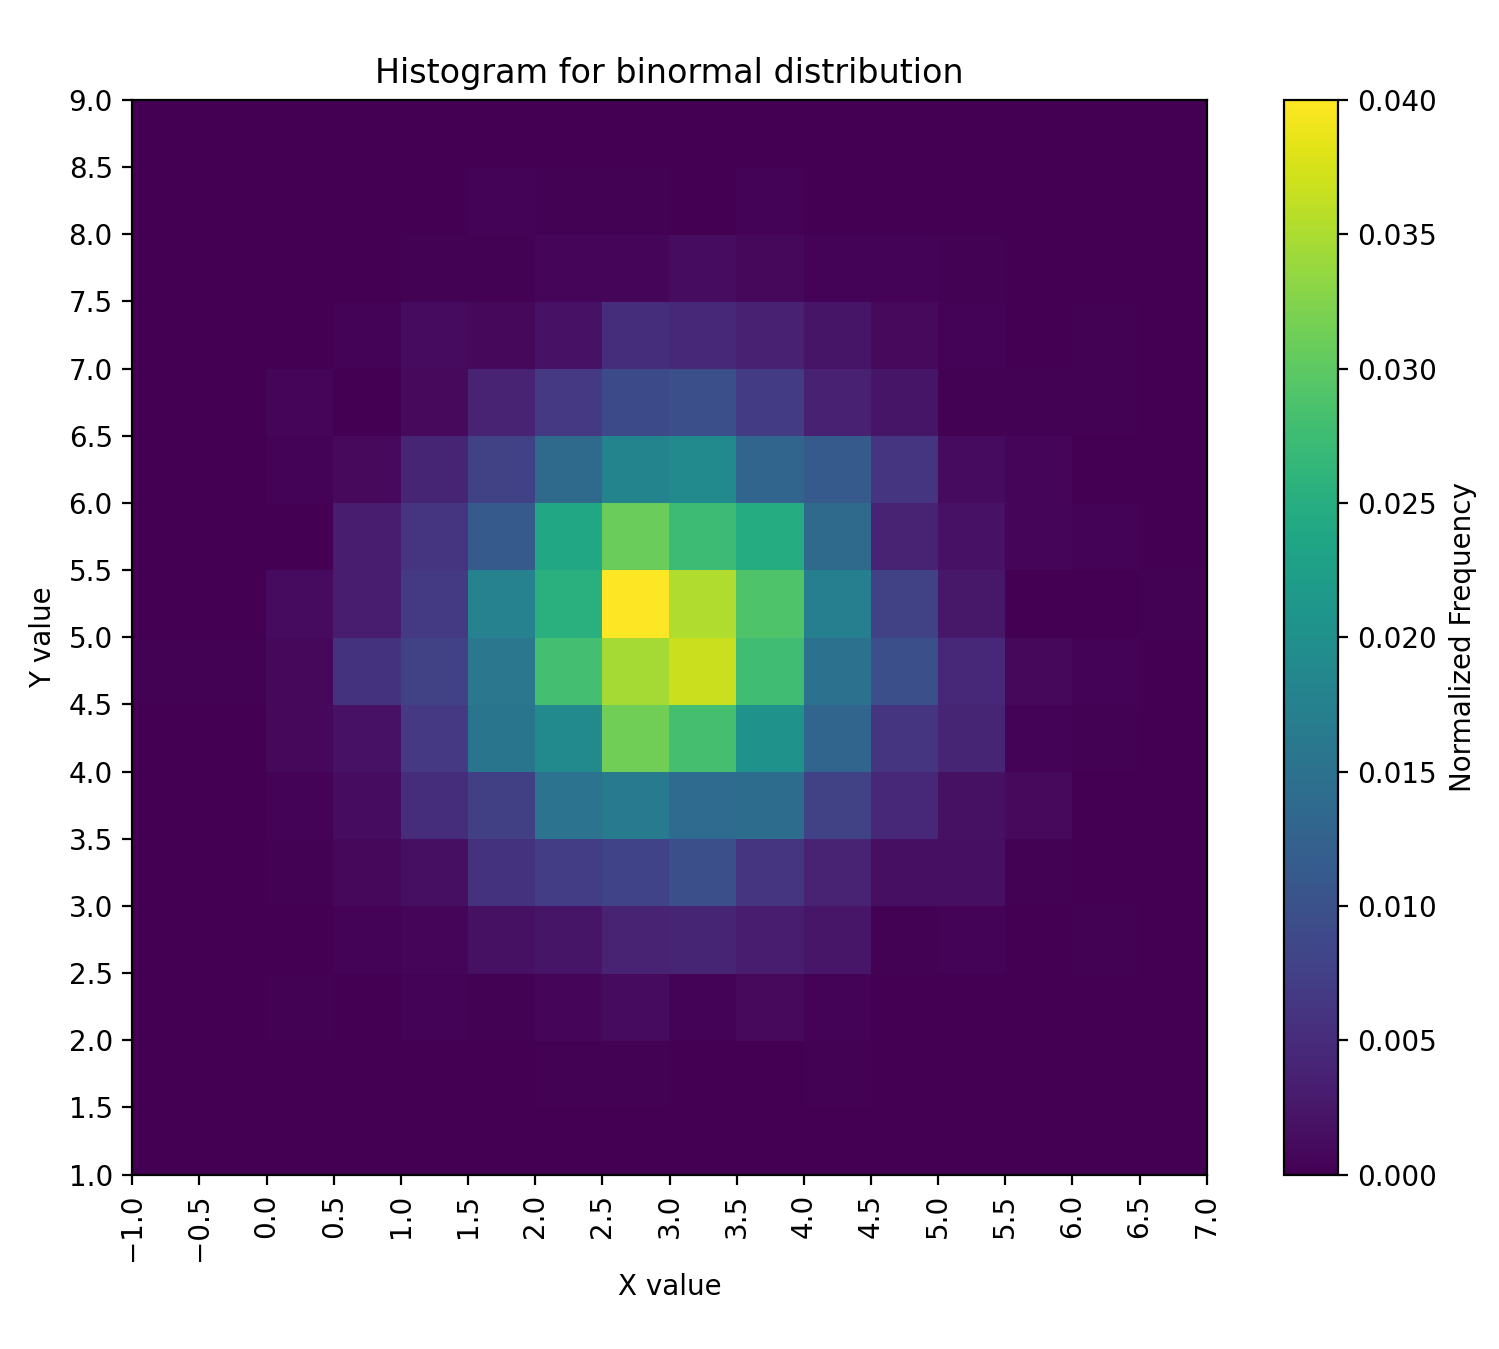
\includegraphics[scale=0.4]{2Dhist.png} 
        \end{minipage}
    }
    \subfigure[Histogram for binormal distribution with $z$] %第二张子图
    {
        \begin{minipage}{8cm}
            \centering      %子图居中
            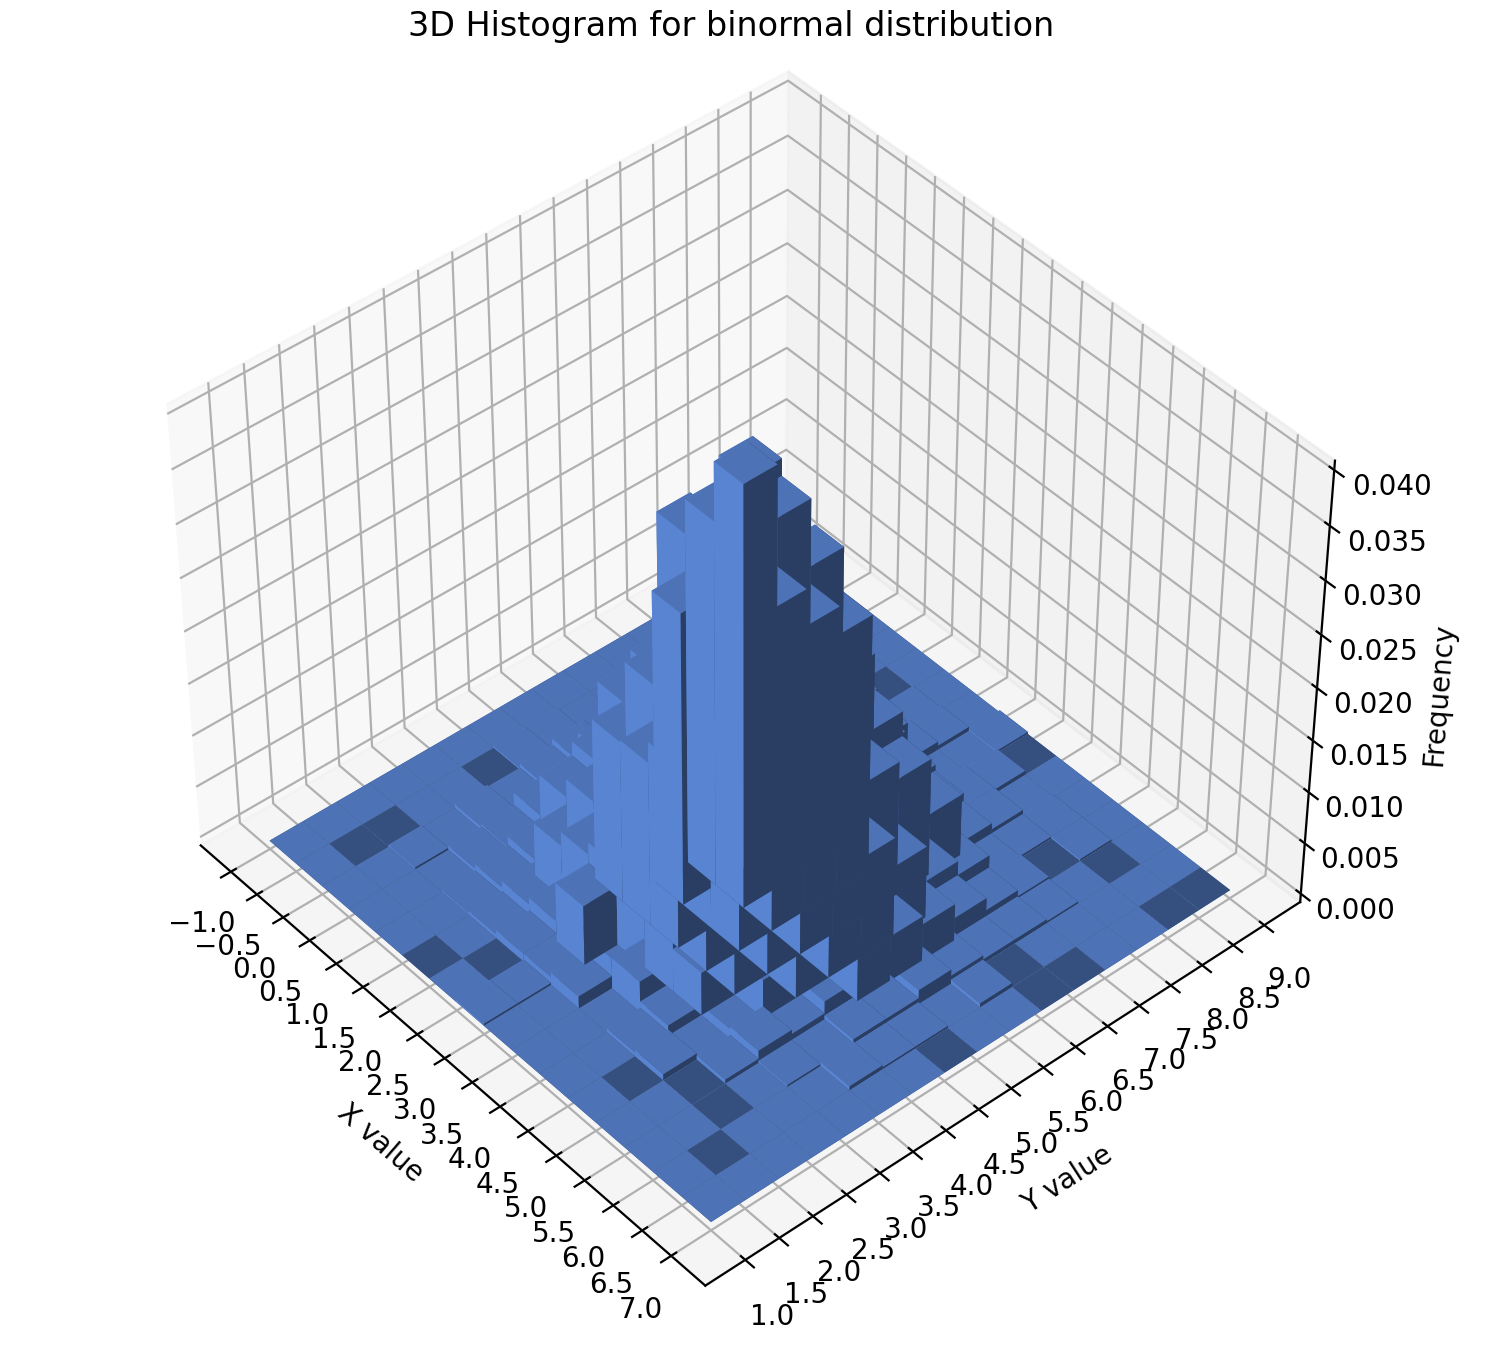
\includegraphics[scale=0.4]{3Dhist.png}
        \end{minipage}
    }
	\caption{2D histogram for binormal distribution sample} %  %大图名称
\end{figure}

\newpage
(2) See localhist\_compute.py
\begin{lstlisting}
from PIL import Image

def local_histogram(img_path):
    '''
    Calculates local histogram of each pixel with a 3x3 neighborhood efficiently using sliding window in a Z-shaped pattern.

    Parameters:
        - img_path: path to input image.
    Returns:
        - local_hist_array: 2D array of dictionaries where each dictionary is a histogram of the 3x3 neighborhood of a pixel.
            - local_hist_array[i][j] is a dictionary of the histogram of the 3x3 neighborhood of the pixel at (j, i).
                    The keys are the pixel values in the neighborhood and their values are the counts of those pixels. Exclude the zero-count pixels.
    '''
    img = Image.open(img_path)
    if img.mode != 'L':
        img = img.convert('L')

    width, height = img.size
    pixels = img.load()

    # Create a 2D array to store the local histograms
    local_hist_array = [[{} for _ in range(width)] for _ in range(height)]

    i, j = 0, 0
    while 0 <= i < height and 0 <= j < width:
        if i == 0 and j == 0:  # Initialize the first histogram manually
            histogram = {}
            for x in [0, 1]:
                for y in [0, 1]:
                    if i + x < height and j + y < width:
                        pixel_value = pixels[j + y, i + x]
                        histogram[pixel_value] = histogram.get(pixel_value, 0) + 1
            local_hist_array[i][j] = histogram

        # Move to the next pixel
        j = j + 1 if i % 2 == 0 else j - 1
        
        # Check if we need to move down or continue horizontally
        move_down = False
        if i % 2 == 0:
            if j == width:  # Reach the end of even row
                i += 1
                j -= 1
                move_down = True
        else:
            if j == -1:  # Reach the start of odd row
                i += 1
                j += 1
                move_down = True
                
        # Update the histogram based on the movement
        if move_down:
            if i == height:  # Reach the end of the image
                break
            else:  # Move down
                histogram = local_hist_array[i-1][j].copy()
                # Adjust for the row that's moved out of the window
                if i-2 >= 0:
                    for y in [-1, 0, 1]:
                        nj = j + y
                        if 0 <= nj < width:
                            pixel_value = pixels[nj, i-2]
                            histogram[pixel_value] -= 1
                            if histogram[pixel_value] == 0:
                                del histogram[pixel_value]

                # Adjust for the row that's moved into the window
                if i+1 < height:
                    for y in [-1, 0, 1]:
                        nj = j + y
                        if 0 <= nj < width:
                            pixel_value = pixels[nj, i+1]
                            histogram[pixel_value] = histogram.get(pixel_value, 0) + 1

            
        else:  # Continue horizontally
            if i % 2 == 0:  # Even row
                prev_j = j - 1
                remove_col = j - 2
                add_col = j + 1
            else:  # Odd row
                prev_j = j + 1
                remove_col = j + 2
                add_col = j - 1
        
            histogram = local_hist_array[i][prev_j].copy()
            
            # Adjust for the column that's moved out of the window
            if 0 <= remove_col < width: # Check if we do not go out of bounds
                for x in [-1, 0, 1]:
                    ni = i + x
                    if 0 <= ni < height:
                        pixel_value = pixels[remove_col, ni]
                        histogram[pixel_value] -= 1
                        if histogram[pixel_value] == 0:
                            del histogram[pixel_value]

            # Adjust for the column that's moved into the window
            if 0 <= add_col < width:  # Check if we do not go out of bounds
                for x in [-1, 0, 1]:
                    ni = i + x
                    if 0 <= ni < height:
                        pixel_value = pixels[add_col, ni]
                        histogram[pixel_value] = histogram.get(pixel_value, 0) + 1

        local_hist_array[i][j] = histogram
    
    return local_hist_array
\end{lstlisting}
\textbf{Code interpretation}:\\
The code above defines a function to calculate local histogram of each pixel with a $3\times3$ neighborhood efficiently using sliding window in a Z-shaped pattern.
The function takes in an image path, and returns a 2D array of dictionaries where each dictionary contains the intensities in the pixel's neighborhood and their counts.\\
The movement process is as follows. Firstly, we initialize the first histogram manually. Then we move on horizontally to the next pixel. If the current row is even, we move to the right. If the current row is odd, we move to the left.
The horizontal move histogram update is done by copying the previous histogram and adjusting for the column that's moved out of the window and the column that's moved into the window.
Whenever we subtract a count from the histogram, we check if the count is zero. If so, we delete the key-value pair from the dictionary in order to save space.\\
However, if we reach the end of the row, we choose to move straight down to the next row. The vertical move histogram update is also done by copying the previous histogram and adjusting for the row that's moved out of the window and the row that's moved into the window.\\
If we reach the end of the image, we break the loop and return the local histogram array.\\

\section{}
Implement the algorithm of local histogram equalization:\\
(1) First implement histogram equalization algorithm, and then\\
(2) implement the local histogram equalization using efficient computation of local histogram.\\
Please test your code on images and show the results in your report.\\
\textbf{Solution}:\\
(1) See hist\_equal.py
\begin{lstlisting}
from PIL import Image
import numpy as np

def histogram_equalization(img_path, L=256):
    '''
    global histogram equalization.
    
    Parameters:
        - img_path: path to input image.
        - L: Number of intensity levels.
    Returns:
        - s_dict: dictionary of equalized intensity values. The keys are original intensities, and the values are equalized intensities.
    '''

    r_dict = intensity_count(img_path,L)
    # calculate the cumulative distribution function
    cdf = np.cumsum(list(r_dict.values()))
    # calculate the equalized intensity s, in a dictionary
    s_dict = {i: round((L-1)*cdf[i]/cdf[-1]) for i in range(L)}
    
    return s_dict

def intensity_count(img_path, L=256):
    '''
    count the number of pixels for each intensity level.
    
    Parameters:
        - img_path: path to input image.
        - L: Number of intensity levels, default is 256.
    Returns:
        - count_dict: dictionary with intensity as key and count as value.
    '''
    # open image
    img = Image.open(img_path)
    
    # convert to grayscale if not already
    if img.mode != 'L':
        img = img.convert('L')
    
    # get pixel values
    pixels = list(img.getdata())

    # initialize dictionary
    count_dict = {i: 0 for i in range(L)}

    # count the number of pixels for each intensity
    for pixel in pixels:
        if pixel in count_dict:
            count_dict[pixel] += 1

    return count_dict


# test the function
# open image
img_path = '.\HW1\moon.tif'
img = Image.open(img_path)

# convert to grayscale if not already
if img.mode != 'L':
    img = img.convert('L')
    
# apply the function
pixels = img.load()
s = histogram_equalization(img_path)
for i in range(img.width):
    for j in range(img.height):
        intensity = pixels[i, j]
        pixels[i, j] = s[intensity]

# save the modified image
img_out_path = ".\HW1\moon_hist_equal.tif"
img.save(img_out_path)
print("Image saved to: {}".format(img_out_path))
\end{lstlisting}
\textbf{Code interpretation}:\\
The code above defines a function to perform global histogram equalization. The function takes in an image path and the number of intensity levels, and returns a dictionary of equalized intensity values.\\
The function first counts the number of pixels for each intensity level, then calculates the cumulative distribution function and equalized intensity values. It applies the equalized intensity values to every pixel value, and saves the modified image.\\
\textbf{Result}:\\
The input original image and the output image after global histogram equalization are shown below in Figure 3. We can see that the low contrast region of the image is improved, but the overall result is an image with a light, washed-out appearance, not very natural.\\
\begin{figure}[htbp]	
    \subfigure[Input original image] %第一张子图
    {
        \begin{minipage}{8cm}
            \centering          %子图居中
            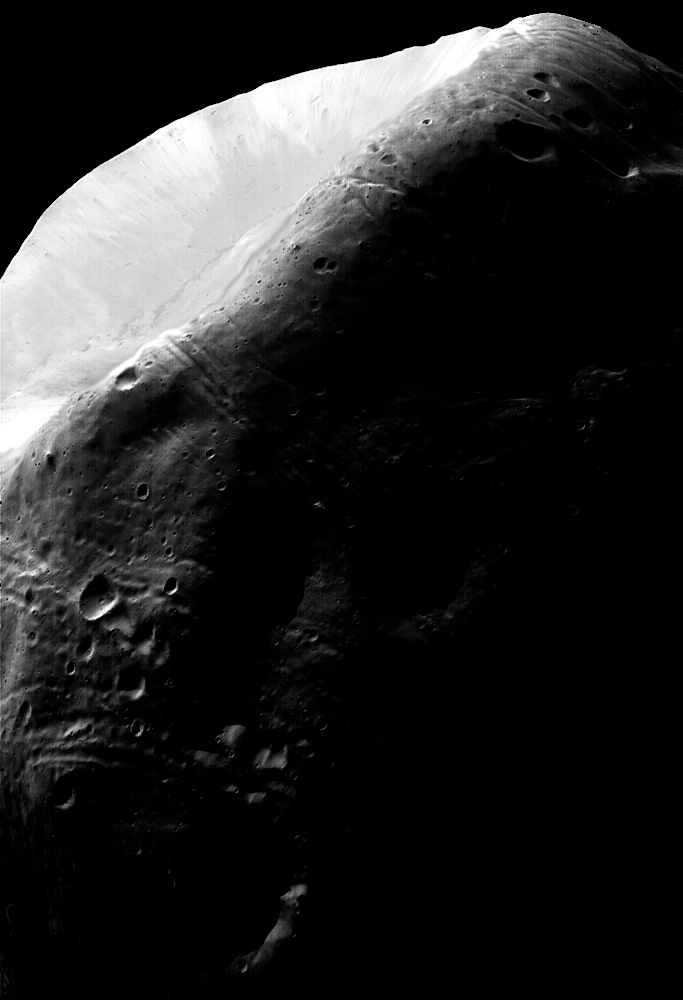
\includegraphics[scale=0.24]{moon.jpg} 
        \end{minipage}
    }
    \subfigure[Output image] %第二张子图
    {
        \begin{minipage}{8cm}
            \centering      %子图居中
            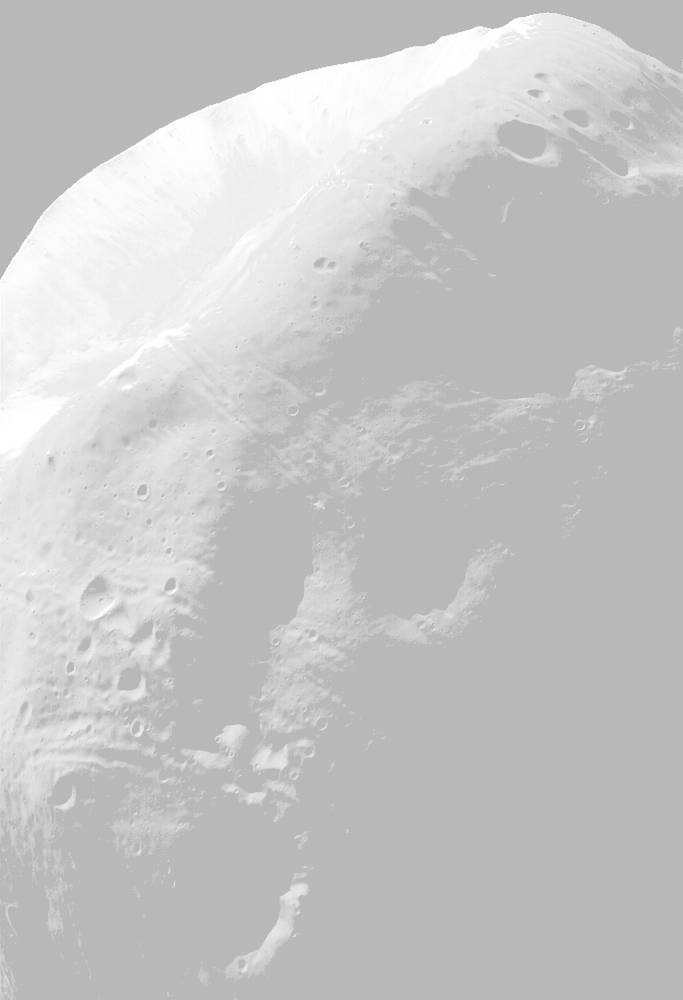
\includegraphics[scale=0.24]{moon_hist_equal.jpg}
        \end{minipage}
    }
    \caption{Image after global histogram equalization} %  %大图名称
\end{figure}

\newpage
(2) See localhist\_equal.py
\begin{lstlisting}
from PIL import Image
from localhist_compute import local_histogram
import numpy as np

def local_histogram_equalization(img_path, L=256):

    '''
    Local histogram equalization based on 3x3 neighborhood.
    
    Parameters:
        - img_path: path to input image.
        - L: Number of intensity levels.
    Returns:
        - s_all: A 2D array consists of equalized intensity values in each position (i,j).
    '''
    
    # open image
    img = Image.open(img_path)
    
    # convert to grayscale if not already
    if img.mode != 'L':
        img = img.convert('L')

    # Get image size and pixels
    width, height = img.size
    pixels = img.load()

    # Calculate local histograms
    local_hist_array = local_histogram(img_path)
    
    # Create a 2D array to store the equalization result
    s_all = [[0 for _ in range(width)] for _ in range(height)]

    for i in range(height):
        for j in range(width):
            # Get the local histogram
            centerintensity = pixels[j, i]
            local_hist = local_hist_array[i][j]
            # Calculate the equalized value for the current pixel based on the local histogram
            s_all[i][j] = local_euqal_calc(local_hist, centerintensity, L)

    return s_all

def local_euqal_calc(local_hist, intensity, L=256):
    '''
    Modified histogram equalization based on given histogram dictionary with count.
    
    Parameters:
        - local_hist: Local histogram dictionary.
        - intensity: Intensity of the neighborhood center.
        - L: Number of intensity levels, default to 256.
    Returns:
        - s: equalized intensity of the neighborhood center.
    '''
    
    # Compute cumulative distribution function
    local_hist = dict(sorted(local_hist.items()))
    cdf = np.cumsum(list(local_hist.values()))
    
    # Calculate the equalized intensity s
    k = 0
    for i in local_hist.keys():
        if i == intensity:
            s = round((256-1)*cdf[k]/cdf[-1])
        k += 1
    return s

# test the function
# open image
img_path = '.\HW1\square_noise.tif'
img = Image.open(img_path)

# convert to grayscale if not already
if img.mode != 'L':
    img = img.convert('L')
    
# apply the function
pixels = img.load()
s_all = local_histogram_equalization(img_path)
for i in range(img.height):
    for j in range(img.width):
        pixels[j, i] = s_all[i][j]

# save the modified image
img_out_path = ".\HW1\square_local_equal.tif"
img.save(img_out_path)
print("Image saved to: {}".format(img_out_path))
\end{lstlisting}
\textbf{Code interpretation}:\\
The code above defines a function to perform local histogram equalization based on $3\times3$ neighborhood. 
The function takes in an image path and the number of intensity levels, and returns a 2D array consists of equalized intensity values in each position $(i,j)$.\\
The function first calculates the local histograms using the function defined in 2(2), then applies the local histogram equalization to every neighborhood center based on the cdf of its neighborhood, and saves the modified image.\\
\textbf{Result}:\\
To test the function and compare the result with global histogram equalization, we use a slightly noisy image with invisible object information. The result is shown below in Figure 4.\\
We can see that global histogram equalization does not work well on this image, for it enhances the noise without revealing the object information clearly; 
while local histogram equalization works better. We can see significant object detail within all the dark squares.
This is mainly because the intensity values of these objects are too close to the intensity of the dark squares, and their sizes are too small to influence global histogram equalization significantly enough to show this level of intensity detail.
Local histogram equalization is based on the local information of each pixel, and thus can enhance the contrast of each pixel more accurately.
\begin{figure}[htbp]	
    \subfigure[Input original image] %第一张子图
    {
        \begin{minipage}{8cm}
            \centering          %子图居中
            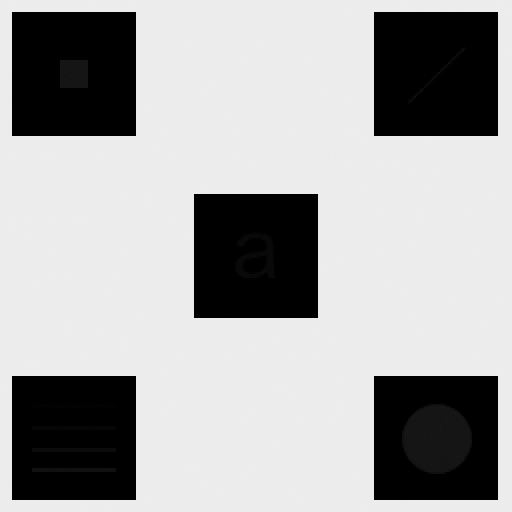
\includegraphics[scale=0.35]{square_noise.jpg} 
        \end{minipage}
    }
    \subfigure[Global histogram equalization] %第二张子图
    {
        \begin{minipage}{8cm}
            \centering      %子图居中
            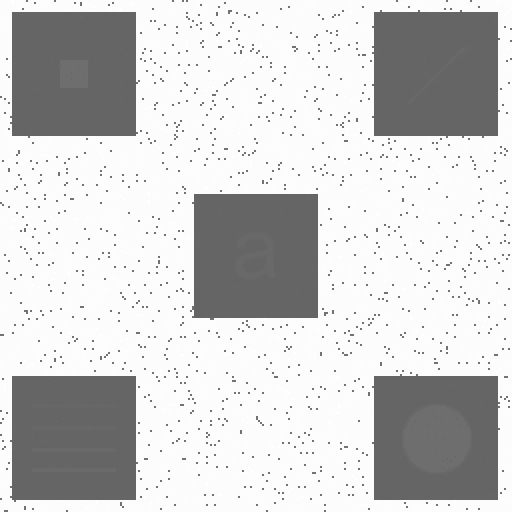
\includegraphics[scale=0.35]{square_hist_equal.jpg}
        \end{minipage}
    }
    \subfigure[Local histogram equalization] %第三张子图
    {
        \begin{minipage}{8cm}
            \centering      %子图居中
            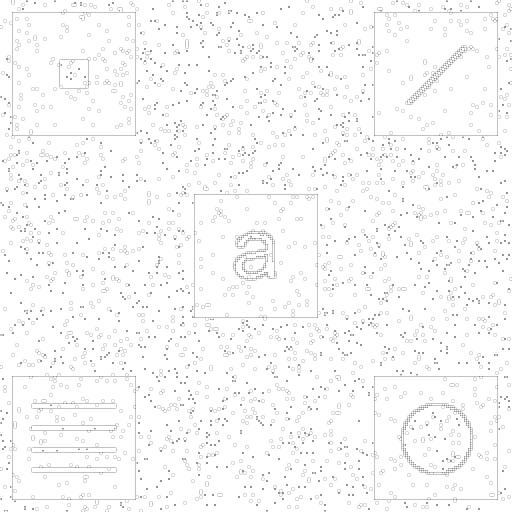
\includegraphics[scale=0.35]{square_local_equal.jpg}
        \end{minipage}
    }
    \caption{Image after global and histogram equalization} %  %大图名称
\end{figure}
\end{document}